\chapter{Introduction}
\section{Motivation}
Whether it be water in a pipeline, or an aircraft soaring through the skies, every fluid passing by a solid and every solid passing through a fluid will experience drag. The ever pressing need to reduce our impact on the environment requires us to reduce our energy used to combat unwanted drag, which also has the added benefit of reducing costs via increased efficiency. This is especially true in the transportation sector, which accounts for 24\% of total global emissions in 2019 according to the IEA, although growth has been limited to only 0.5\% per year compared to an average increase of 1.9\% annually since 2000 owing to efficiency improvements \cite{iea2021}.

The search for these efficiency improvements includes research towards \gls{dr} via flow control -- that is manipulating the flow characteristics in such a way that somehow produces less overall drag. In fact, Ludwig Prandtl, who revolutionised the study of fluid mechanics with the introduction of the \gls{tbl}, pioneered modern flow control as early as 1904, where he demonstrated that suction at the surface of a cylinder delays \gls{bl} separation and therefore decreases drag \cite{gad-el-hak2001,prandtl1904}. Indeed, \gls{dr} is a major focus of research in commercial aviation. In the context of aviation, a 1\% reduction in drag corresponds to a 0.75\% reduction in fuel and as a result \ensuremath{\mathrm{CO_2}} emissions \cite{leschziner2011}. In fact, \cite{leschziner2011} states that based on estimates on travel demand in 2030, a 1\% reduction will constitute a 9 million tonnes reduction in \ensuremath{\mathrm{CO_2}} emissions.

In transport applications, and in particular aviation, the flows are at high Reynolds numbers \gls{re}, this means the regimes we are dealing with are often turbulent. Moreover, especially in aviation (with the exception of cases where supersonic effects dominate), viscous drag generated in the near-wall \gls{bl} region constitutes a major component of total drag \cite{abbas2017}. These two factors combined mean that ``flow control methodology targeting the \gls{tbl} is the most obvious option to achieve a significant skin-friction-drag reduction and ultimately to reduce emissions" \cite{abbas2017}.

Flow control is separated into two distinct groups, active and passive control. Active flow control requires an input in energy to affect the flow via the use of actuators, whereas passive flow control does not. Examples of active control include opposition control \cite{choi1994,luhar2014}, spanwise-wall oscillation \cite{jung1992,choi1998,viotti2009}, and the aforementioned \gls{bl} separation control \cite{prandtl1904}; the former is closed-loop and reacts to sensor inputs from the environment, whereas the latter two can be either open-loop with predetermined control patterns or reactive (feedback/feed-forward systems). The actuators used to perform active flow control can range from zero-net-mass-flux jets \cite{zhang2008}, to dielectric-barrier-discharge plasma actuators \cite{wang2013}, to fluid injection (blowing) and sucking \cite{chng2009}, to the ingenious moving surface using ``pneumatically actuated compliant structure based on the kagome lattice geometry'' \cite{bird2018}.
Whereas, examples of passive control include vortex generators \cite{chang1970}, discontinuities/notches/fences in the leading/rear edges of a wing \cite{chang1970}, compliant surfaces \cite{choi1997}, porous coatings \cite{klausmann2017}, superhydrophobic surfaces \cite{truesdell2006}, and a very well studied control technique known as riblets \cite{walsh1983,choi1993,garcia-mayoral2011}.

As aforementioned, active flow control allows for reactive responses which can increase the effectiveness of control techniques. Moreover, even open-loop flow control can achieve higher viscous drag reduction than passive control techniques without the need for sensors required for reactive flow control. However, this comes at a cost of the extra energy expended to modify the flow and the difficulty and innovation needed to design actuators. This can clearly be seen in the case of spanwise-wall oscillation where the wall moves as prescribed by a streamwise travelling wave, which, after accounting for the power spent to oscillate the fluid, has a net power saving of around 26\% despite a drag reduction of $>35\%$ for those conditions \cite{quadrio2009}. Moreover, in order to emulate a in-plane wall motion in real life, the aforementioned compliant structure from \cite{bird2018} had to be created and trialled in laboratory conditions, and then made at scale and maintained if it were to be used on real-world flows.

On the other hand, passive flow control in necessarily open-loop, and may have decreased performance in comparison to active flow control. However, it does not require actuators and the maintenance thereof. Riblets, for example, ``are small surface protrusions aligned with the direction of the flow, which confer an anisotropic roughness to a surface'' \cite{garcia-mayoral2011} and can be seen in Figure~\ref{fig:riblets}. Experiments show that under moderate adverse pressure gradient (i.e. where the pressure increases along the direction of the flow) a 13\% skin friction reduction is achievable, compared to 6\% reduction in a zero-pressure-gradient \gls{bl} \cite{debisschop1996}. Although less efficient compared to active control, due to its relatively simple design, its \gls{trl} is higher than most other flow control techniques. In fact it has been trialled in scale model aircraft tests in transonic Mach numbers \cite{coustols1990}, real aircraft tests, and even in commercial service for several years by Cathay Pacific on an Airbus A340 where 30\% of the wetted surface was covered with riblets \cite{bechert2006}. Based on a flight test on an Airbus A320, in transonic Mach number ranges, an A320 with 70\% of the wetted surface covered by riblets could have a drag reduction of about 2\% \cite{szodruch1991}. However, the optimal grove cross section was found to have an optimum at $\gls{gA}^{1 /2}\approx11$, where the $+$ superscript denotes non-dimensionalisation by wall units (see \ref{ssec:ssl}) and spacing of approximately 15 wall units \cite{garcia-mayoral2011}. This is equivalent to approximately \SIrange{30}{70}{\micro\metre} in realistic aerofoil and aircraft flows \cite{garcia-mayoral2011}. Moreover, the sharper the riblets, the more efficient they are at reducing drag \cite{garcia-mayoral2011}. All of these factors make riblets quite hard to manufacture whilst requiring maintenance/replacements due to the erosion from air moving past.

\begin{figure}[htbp]
\centering
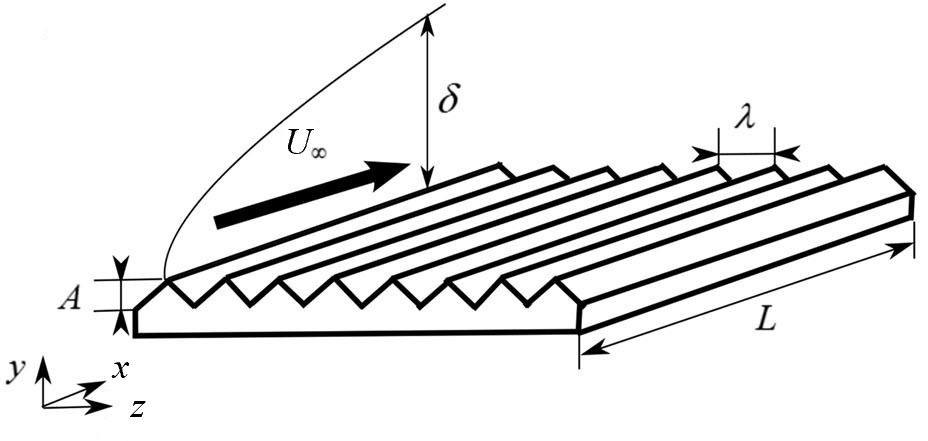
\includegraphics[width=0.5\linewidth]{introduction/fig/riblets.jpeg}
\caption{A schematic of triangular riblets the most commonly researched riblets. Figure modified from \cite{raayai-ardakani2019}.}
\label{fig:riblets}
\end{figure}

Therefore, researchers have begun to explore other ways to use passive flow control for turbulent \gls{dr}. The oblique \gls{ww} was first proposed by \textcite{chernyshenko2013} in 2013 to emulate the motions of in-plane spanwise wall oscillations in hopes that there will be a net energy decrease. We will devote the rest of this report discussing the merits of this curious passive flow control method. 



%It is known that if in a turbulent flow the (wing) surface moves spanwise with a suitable velocity distribution, the friction drag is significantly reduced. Even though causing the wing surface to move requires energy input, the drag reduction is large enough to provide large energy savings. However, such motion is difficult to implement on an aircraft. In a paper (Chernyshenko, 2013, arxiv.org/abs/1304.4638) it was proposed to shape the rigid (not moving) surface in such a way that the resulting fluid motion will emulate the effect of the surface motion without the surface actually moving. For the case of the surface with sinusoidal waves at an angle to the mean flow direction, an optimisation of the angle and the height of the waves was performed. The later comparisons (Ghebali et al., 2017, aip.scitation.org/doi/10.1063/1.5003617) showed that the semi-empirical model of calculating the drag reduction used for optimisation was inaccurate. This might be due to this model not taking into account the energy dissipation due to the laminar viscosity and the shape of the mean velocity profile. This part of the dissipation is negligible at high Reynolds numbers, but it was significant at the Reynolds numbers studied. The project will consist in improving the semi-empirical model and repeating the shape optimisation using the improved model. It is recommended to see the first paper cited above to estimate the degree of mathematical proficiency needed for this project.
\section{Literature Review}
\subsection{The Spatial Stokes Layer (SSL)}\label{ssec:ssl}
The Stokes layer is one of a few exact solutiosn to the Navier-Stokes equation describing the motion of a viscous fluid as a function of the wall normal coordinate $y$, whereby the infinitely long wall is located at the bottom at $y=0$ and oscillating harmonically in its own plane \cite{schlichting2017}. It turns out that the resulting oscillation in the fluid is only of significant magnitude very close to the wall in a so-called ``Stokes layer'' and is significantly damped outside of the said-layer.

\citeauthor*{jung1992} \cite{jung1992} were the first to suggest using a wall oscillating in the spanwise direction to reduce skin friction in 1992, exploiting the above phenomenon to obtain a maximum drag reduction of 40\% at a non-dimensional period of $T^+=100$ using \gls{dns}, a \gls{cfd} method \cite{karniadakis2003}. The $+$ superscript denotes non-dimensionalisation by wall units, which is based upon the wall friction velocity $\gls{ut}=\sqrt{\frac{\gls{tw}}{\gls{ro}}}$, along with the kinematic viscosity $\gls{nu}=\frac{\gls{mu}}{\gls{ro}},$ where \gls{tw} is the wall shear stress of the fluid flow, \gls{ro} is the density of the fluid, and \gls{mu} is the dynamic viscosity of the fluid flow. The spanwise velocity of the wall is given by
\begin{equation}
	\gls{spanwv} = \gls{awall}\sin{\left( \frac{2\pi}{\gls{per}}\gls{tim} \right) 
,\end{equation}
where \gls{awall} and \gls{per} denotes the oscillation amplitude and period, and \gls{tim} denotes time.
Moreover, when only one of the channel walls were oscillating, ``the reduction in turbulence activity was observed only near the oscillating wall, while the flow at the other wall remained fully turbulent'' \cite{jung1992}. When phase averaged this coincides with the Stokes layer with temporal forcing \cite{viotti2009}, we will therefore name it \gls{tsl}. \textcite{dhanak1999} observed that the duration of sweep events were reduced by 47\% and their strength reduced by 23\%, suggesting that the skin-friction reduction is a result of the ``attenuation in the formation of streamwise streaks \cite{karniadakis2003}.
%\textcite{karniadakis2003} provides an excellent review of research in in-plane wall motion up to 2003. 

As this is a form of active flow control, despite significant drag reductions, significant energy must also be expended to overcome the extra shear stress to create the spanwise motion of the fluid \cite{viotti2009}. \textcite{baron1996} was the first to consider the net energy savings from spanwise wall oscillation, and it is now accepted that the net energy savings is 10\% \cite{viotti2009, karniadakis2003}. However, this technique requires moving parts and therefore requires actuators, which is hard to implement in practical applications especially in transport applications.

\textcite{viotti2009} sought to extend the \gls{tsl} from a time-dependent forcing to a stationary, spatial forcing, which potentially allows an extension into passive solutions which can emulate the oscillation varying over space instead of time (such as the \gls{ww}). (------------------------------------------------------------------------------------------------------------------------------------------ kim and hussain--------------------------------???)
The spatial forcing law can be seen in Figure~\ref{fig:ssl}, and is given by
\begin{equation}
	\gls{spanwv} = \gls{awall}\sin{\left( \frac{2\pi}{\gls{lm}_x} x \right)} 
,\end{equation}
where $\gls{lm}_x$ denotes the forcing wavelength in the streamwise coordinate $x$. We will call this the \gls{ssl}.

\begin{figure}[htbp]
\centering
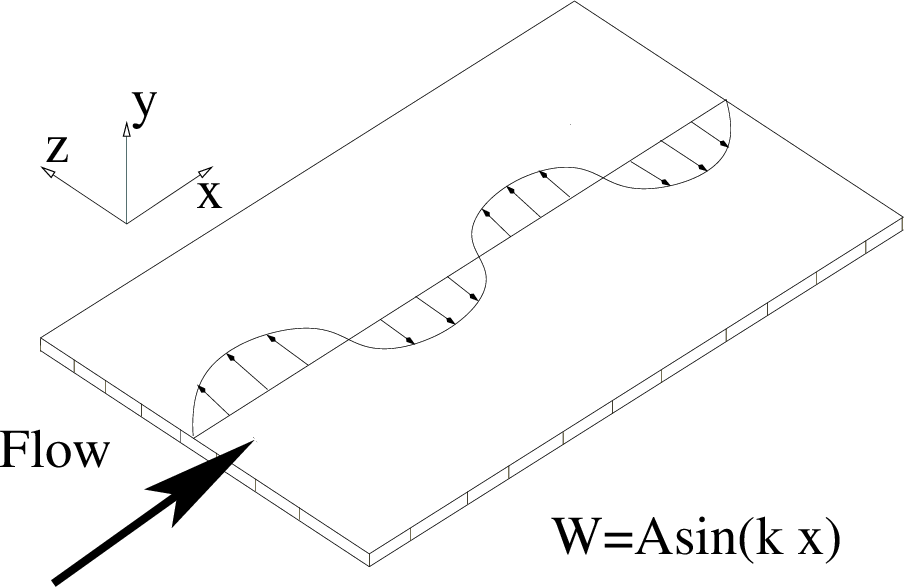
\includegraphics[width=0.5\linewidth]{introduction/fig/ssl.png}
\caption{Schematic of spanwise wall forcing from \cite{viotti2009}. }
\label{fig:ssl}
\end{figure}

We will now analyse \gls{ssl} flow analytically following \textcite{chernyshenko2013}, who ultimately derives their analysis from \textcite{viotti2009}. We begin with the triple decomposition of velocity as follows
\begin{equation}
	\mathbf{U} = \overline{\mathbf{U} }+\tilde{\mathbf{U} }+\mathbf{u'}  
,\end{equation}
where $\overline{\mathbf{U} }$ is the velocity averaged over time, and space in the $x$ and  $z$ direction, $\tilde{\mathbf{U} }$ is the phase averaged velocity, and $\mathbf{u'} $ is the remaining stochastic turbulent part of the velocity. Unlike the traditional Reynolds decomposition, we have an extra phase dependent term, which is useful for periodic flows such as \gls{ssl} flow. We can adapt the definition given in \cite{baj2015} to our case and define for some phase angle $\gls{phase}_0=\gls{phase}(x_0+m \gls{lm}_x,z_0+n \gls{lm}_z)$,
\begin{equation}
	\tilde{\mathbf{U} }(y,\gls{phase}_0):=\lim_{M\to\infty}\lim_{N\to\infty}\frac{1}{M}\frac{1}{N} \sum_{m=1}^{M} \sum_{n=1}^{N} \mathbf{U}(x_0+n \gls{lm}_x,y,z_0 +m \gls{lm}_z)-\overline{\mathbf{U} }(y)  
.\end{equation}
By including this average, we recognise that there will be periodicity in the $x$ component of the flow velocity; we also include periodicity in the $z$ component of the flow velocity since it will be useful for the \gls{ww} flow, and doesn't affect the definition for the \gls{ssl} flow, whose phase average has no $z$ dependence and therefore $\tilde{W}=0$.

With that definition, we can now solve for the phase averaged velocity of the \gls{ssl} flow. By linearising the \gls{bl} equations in the wall units of the flow around a linear profile, we ignore the stochastic fluctuations $\mathbf{u'} $ and let $\overline{\mathbf{U} } = (y,0,0)$. Moreover, \gls{ssl} is time invariant. Thus, by analysing the order of various values as in \cite{schlichting2017}, and taking $\gls{re}\to \infty$, we get
\begin{align}
	y^{+} \pdv{\tilde{U}^{+}}{x^{+}} + \tilde{V}^{+} &= -\pdv{p^{+}}{x^{+}} + \pdv[2]{\tilde{U}^{+}}{y^{+}} \\
	0 &= -\pdv{p^{+}}{y^{+}}  \\
	y^{+} \pdv{\tilde{W}^{+}}{x^{+}} &= -\pdv{p^{+}}{z^{+}} + \pdv[2]{\tilde{W}^{+}}{y^{+}} \\
	0 &= \pdv{\tilde{U}^{+}}{x^{+}} +\pdv{\tilde{V}^{+}}{y^{+}} +\pdv{\tilde{W}^{+}}{z^{+}} 
.\end{align}

At the wall ($y^{+}=0$),  $\tilde{U}^{+}=\tilde{V}^{+}=0$, and $\tilde{W}^{+}=\gls{awall}e^{i \gls{wnum}_x x}$, where we take the real part only at the end of calculations.

%Intro: Motivation, Riblets, and others in general, Lit Review – Stokes Layer Results; SSL+Chernyshenko. Refer to Ghebali DNS. End:Formulation of problem: want to be able to predict drag reduction by WW as f’n of $k_x, k_z$, and What



%It is known that if in a turbulent flow the (wing) surface moves spanwise with a suitable velocity distribution, the friction drag is significantly reduced. Even though causing the wing surface to move requires energy input, the drag reduction is large enough to provide large energy savings. However, such motion is difficult to implement on an aircraft. In a paper (Chernyshenko, 2013, arxiv.org/abs/1304.4638) it was proposed to shape the rigid (not moving) surface in such a way that the resulting fluid motion will emulate the effect of the surface motion without the surface actually moving. For the case of the surface with sinusoidal waves at an angle to the mean flow direction, an optimisation of the angle and the height of the waves was performed. The later comparisons (Ghebali et al., 2017, aip.scitation.org/doi/10.1063/1.5003617) showed that the semi-empirical model of calculating the drag reduction used for optimisation was inaccurate. This might be due to this model not taking into account the energy dissipation due to the laminar viscosity and the shape of the mean velocity profile. This part of the dissipation is negligible at high Reynolds numbers, but it was significant at the Reynolds numbers studied. The project will consist in improving the semi-empirical model and repeating the shape optimisation using the improved model. It is recommended to see the first paper cited above to estimate the degree of mathematical proficiency needed for this project.


%This is one of the most important components of the dissertation. It should begin with a clear statement of what the project is about so that the nature and scope of the project can be understood by a lay reader. It should summarise everything you set out to achieve, provide a clear summary of the project's background and relevance to other work and give pointers to the remaining sections of the dissertation which contain the bulk of the technical material.
%
%Further information can be found here: \url{https://goo.gl/k2huN9}.
%
%\section{\LaTeX{} code examples and formatting tips}
%Hello, here's a citation \cite{greenwade93}. References are stored in a Bibtex file. Google Scholar and IEEExplore allow you to download citations of papers in Bibtex format from their search engine. Some people use JabRef (\url{http://www.jabref.org}) to manage their database of references.
%
%This is an inline equation $\Gamma(t)=K_i e^{\sin^2(\omega_t)}$. The first paragraph appears without indent but the following ones will have an indentation.
%
%This is an actual named equation:
%\begin{equation}
%v(x)=\frac{1}{2}\sin(2 \omega t + \phi) e^{-j s t}
%\label{eq:cacona}
%\end{equation}
%\noindent where $\omega$ is the angular speed. Notice that symbols liks $\omega$ should be written in italics whereas measurement units such as V for Volts appear as normal text. This paragraph didn't have an indentation because the first sentence was linked to the definition of equation (\ref{eq:cacona}). A code snippet for an example program is shown in Listing~\ref{lst:code1}.
%
%\begin{lstlisting}[caption=Source code for {\it hello.m},label=lst:code1,breaklines=true,basewidth=4pt,prebreak=**,postbreak=**,frame=single]
%for i:=maxint to 0 do
%begin
%{ do nothing }
%end;
%Write('Case insensitive ');
%Write('Pascal keywords.');
%\end{lstlisting}
%
%The characteristic parameters of the system are sumarised in Table~\ref{tab:tab1}. A figure is shown Fig~\ref{fig:felix}, we don't necessarily know if this figure will appear below, above or elsewhere; therefore, the text should never refer to the figure with sentences such as {\it "As shown here:"}.
%%
%\begin{figure}[htbp]
%\centering
%
\includegraphics[width=0.3\linewidth]{introduction/fig/Felix_the_cat.pdf}
%\caption{Felix the Cat}
%\label{fig:felix}
%\end{figure}
%
%\begin{table}[htbp]
%	\centering
%	\begin{tabular}{lll}
%		Parameter & Value & Units\\
%		\hline
%		$P$ & 1 & kW \\
%		$Q$ & 0 & kVAr\\
%	    \hline
%	\end{tabular}
%	\caption{Characteristic parameters of the system}
%	\label{tab:tab1}
%\end{table}
%
%\begin{samepage}
%Sometimes, the symbols in an equation are defined as follows\footnote{Some authors like to define their symbols this way.}:
%\begin{equation}
%	V(t)=A \sin(\omega t+\theta_0)
%\end{equation}
%\begin{tabular}{lll}
%	where & $V$ & is a voltage waveform,\\
%	& $A$ & is the amplitude of the voltage,\\
%	& $\omega$ & is the angular frequency,\\
%	& $t$ & is the time.
%\end{tabular}
%\end{samepage}
%
%\subsection{A brief comparison between a proper plot and a horrible plot}
%
%Figure \ref{fig:fig2} contains two plots of the same waveform. Subfigure \ref{fig:fig2sub1} shows a badly formatted figure, Subfigure \ref{fig:fig2sub2} shows a much better formatted figure. The problems with Subfigure \ref{fig:fig2sub1}, listed by order or relevance, are the following:
%
%\begin{enumerate}
%    \item The font size is too small to be read properly.
%    \item The axes aren't labeled properly: the horizontal axis is not labeled and the units of the vertical axis are unknown. Further, symbols must be written in italics whereas numbers and units must be written as normal text.
%    \item The choice of limits for the axes is not good, the figure has wide useless empty spaces. The most relevant part of the waveform is the transient that happens between times $t=$0 and $t=$0.05 s, which is less than 10\% of the timespan shown in the figure.
%    \item The figure has been scaled without keeping the original aspect ratio and fonts look narrower than they would if the figure had been scaled properly.
%    \item The plot doesn't have grid lines. This makes it hard to read the exact value (ie time, voltage) of points in the trace.
%    \item The width of the trace is too thin and may not be visible if printed in low resolution.
%    \item The choice of units of the vertical axis aren't the best. For example, in this case the plot would be easier to read if voltage had been expressed in kV instead of V.
%    \item The figure was exported as a bitmap (e.g. png, jpg, bmp) instead of being exported in vector format (e.g. eps, svg, pdf) and visual artifacts appear when the figure is scaled up or down in order to fit in the document.
%\end{enumerate}
%
%\begin{figure}[htbp]
%	\centering
%	\subfigure[A horrible one.]{
%		\label{fig:fig2sub1}
%        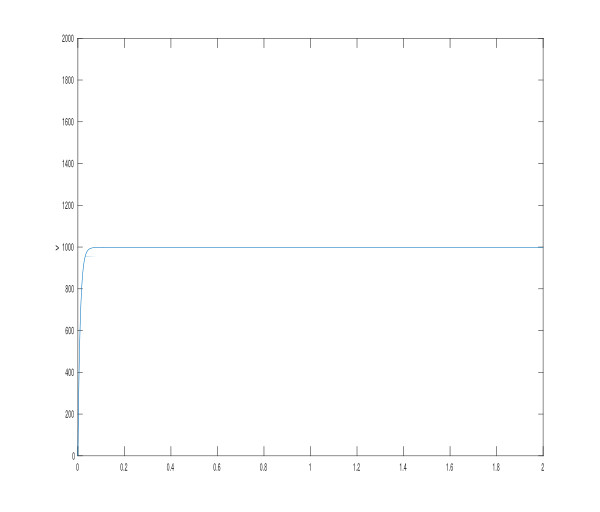
\includegraphics[width=0.5\linewidth]{introduction/fig/figure1.jpg}}
%	\subfigure[A proper one.]{
%		\label{fig:fig2sub2}
%		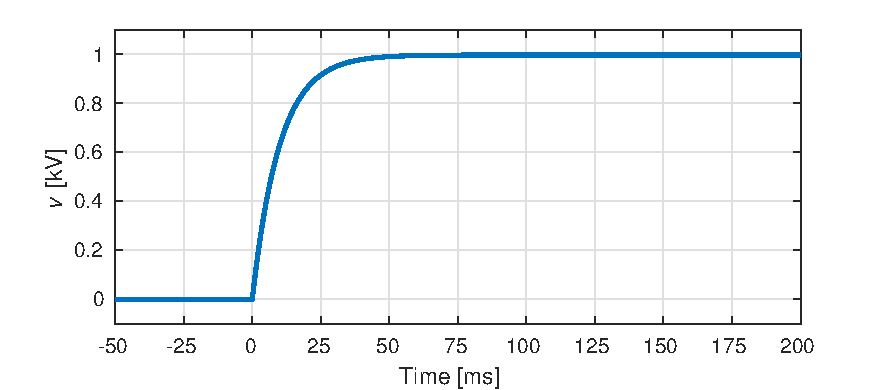
\includegraphics[width=0.6\linewidth]{introduction/fig/figure2.pdf}}
%	\caption{A figure with two subfigures.}
%	\label{fig:fig2}
%\end{figure}
%
%\begin{landscape}
%	\begin{figure}[htbp]
%\centering
%
\includegraphics[width=0.5\linewidth]{introduction/fig/Felix_the_cat.pdf}
%\caption{Here's a large drawing of Felix the Cat that wouldn't fit in a portrait page}
%\label{fig:felix2}
%\end{figure}
%\end{landscape}
%
%\section{Objectives}
%\section{Challenges}
%\section{Contributions}
